
\documentclass[a4paper,12pt]{article}
% \input{../../../config.tex}
\usepackage{../../../../mypackages}
\usepackage{../../../../macros}


\usepackage{pgfplots}
    \pgfplotsset{
    compat=1.11,
  }

\usetikzlibrary{shapes,arrows,babel}
\tikzstyle{box}=[minimum size = 0.1cm, rectangle, draw=black, fill=gray]
% Define the global variable



\begin{document}

\title{Fonctions - Projets de fin de chapitre}
\author{N. Bancel}

\sloppy  % This will apply the sloppy setting to the entire document.
\maketitle

\section{Architecture - L'arche de Saint-Louis}

\begin{tcolorbox}
  \textbf{Notes} : Cet exercice est guidé, et permet de modéliser une structure architecturale avec des fonctions mathématiques. \par
  \vspace{1em}
  Notions abordées :
  \begin{itemize}[noitemsep]
    \item[$\bullet$] Polynôme du second degré
    \item[$\bullet$] Tableau de valeurs
    \item[$\bullet$] Appartenance d'un point à une courbe
  \end{itemize}
  \end{tcolorbox}

Enoncé : faire l'exercice (2) de la page 148 (nommé L'arche de Saint-Louis)


\section{Le pont de San Francisco}

\begin{tcolorbox}
  \textbf{Notes} : Cet exercice est volontairement peu guidé, il nécessite de formuler un problème de manière indépendante. Pour autant : ne pas hésiter à solliciter un/une camarade de classe, ou me solliciter sur Discord. \par
  \vspace{1em}
  Notions abordées :
  \begin{itemize}[noitemsep]
    \item[$\bullet$] Polynôme du second degré et fonctions affines
    \item[$\bullet$] Domaine de définition
    \item[$\bullet$] Modélisation
    \item[$\bullet$] Tableaux de valeurs
    \item[$\bullet$] Mise à l'échelle
  \end{itemize}
  \end{tcolorbox}

  \begin{figure}[H]
    \centering
    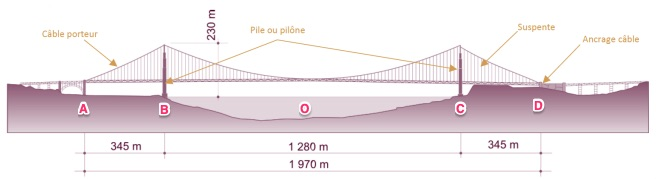
\includegraphics[width=\linewidth]{pont_san_francisco.jpg}
    \caption{\label{} Le pont de San Francisco}
\end{figure}

Nous allons essayer de modéliser le pont de San Francisco (situé entre les points \(A\) et \(D\) sur le plan) avec des fonctions affines et paraboliques. \par
%\vfill
%\break
\vspace{1em}
\textbf{Hypothèses}
\begin{itemize}[noitemsep]
  \item[$\bullet$] On prendra comme origine du repère le point \(O\)
  \item[$\bullet$] Le plateau (qui correspond à la route sur laquelle roulent les voitures) est situé à 60 mètres au dessus de l'eau
  \item[$\bullet$] La fonction entre les points \(A\) et \(B\) peut être modélisée par l'équation \(f(x) = ax+b\)
  \item[$\bullet$] La fonction entre les points \(B\) et \(C\) peut être modélisée par l'équation \(g(x) = cx^2+d\)
  \item[$\bullet$] La fonction entre les points \(C\) et \(D\) peut être modélisée par l'équation \(h(x) = ex+f\) 
\end{itemize}

\textbf{Questions}

\begin{enumerate}[noitemsep, label=(\arabic*)]
  \item Déterminer les équations des fonctions \(f(x)\), \(g(x)\) et \(h(x)\)
  \item Quels sont leurs domaines de définition ?
  \item Représenter ces fonctions sur GeoGebra
  \item En s'aidant d'un tableau de valeurs et des fonctions \(f\), \(g\) et \(h\) définies ci-dessus, dessiner le pont de San Francisco sur un repère dont l'axe des \(x\) mesure 20 cms (et s'étend des graduations -10 à +10)
\end{enumerate}

\end{document}
